\documentclass[main.tex]{subfiles}

\begin{document}

\section{Radiotherapy and Proton Therapy}

\subsection{Radiotherapy}

Cancer is an umbrella term for many diseases involving out-of-control cell growth in the body, the most common types being breast, lung, and prostate cancer\cite{cancerData}. \gls{rt} as treatment started in the early 1900s, using X-rays to malignant tumours, and has become a standard procedure to remove or prevent the growth of malignant tumours. External \gls{rt} uses an external radiation source to deliver the dose. In contrast, internal \gls{rt} injects a radioactive element as a liquid into the body or near the malignant tumour. This thesis will focus on external \gls{rt} methods.
 
 \subsubsection{History and General Use}
 
 \gls{rt} was historically performed by using an external X-ray source and sending the radiation into the patient to treat growths or lesions from diseases such as lupus or skin cancer. \autoref{fig: rt_treatment_history} shows a patient being treated with X-rays before the dangers of radiation therapy was known. Today, the procedure is performed in a similar manner, but better understanding of radiation behaviour and dosage planning enables us to target cancers inside the the patient and better treat life threatening diseases. Imaging techniques such as \gls{ct}-scans allows us to measure the radiodensity of the tissue in a patient, which can be used to create a dosage plan for \gls{rt}. Not only does this allow us to target tumours deep inside the body, but it also allows for higher accuracy dose distribution, which minimizes the amount of radiation absorbed by healthy tissue.
 
  \begin{figure}[!htpb]
    \centering
    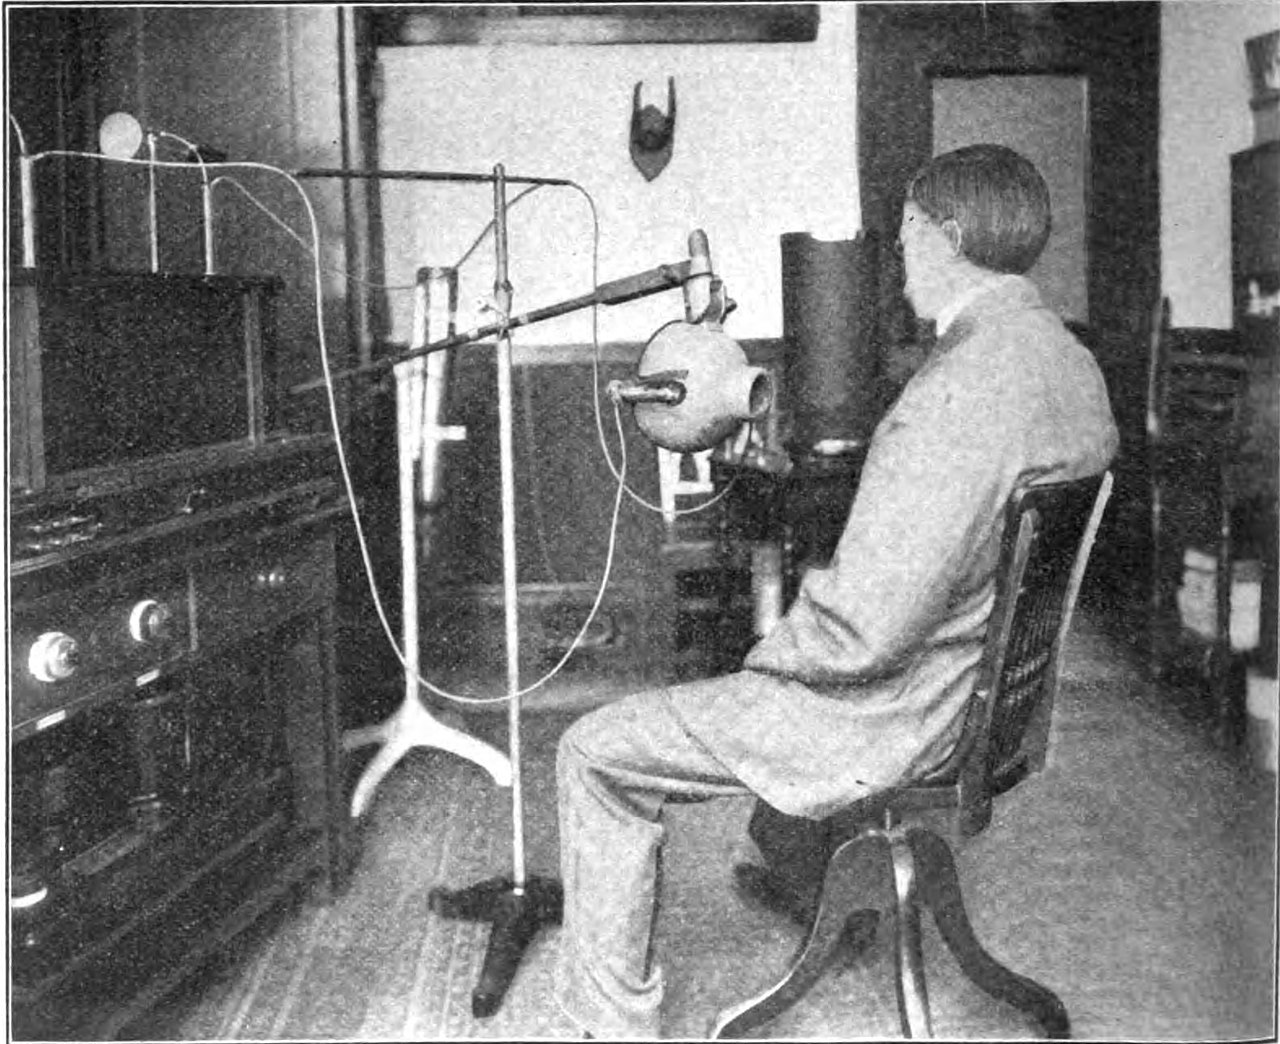
\includegraphics[width=8cm ]{images/x_ray_treatment_history.jpg}
    \caption{Image showing a patient being treated for tuberculosis in 1910, using X-rays.\cite{rt_history}}
    \label{fig: rt_treatment_history}
\end{figure}
 
 Compared to chemotherapy and surgery, \gls{rt} has the advantage of being a non-invasive procedure and can target specific areas in the body. This allows us to remove malignant tumours more effectively and is often used alongside surgery or chemotherapy to ensure the entire tumour is removed. The downside of \gls{rt} is that when the malignant tumour is irradiated, so is the healthy tissue around the tumour, which damages it and can lead to more health issues. Using \gls{rt} in tumours near critical organs, such as the heart or brain, is difficult and must be carefully calibrated to avoid damaging healthy tissue. Using \gls{rt} in areas such as the head and neck has proven to cause many long-term side effects in patients, such as cognitive impairment and neurological damage. In rare instances, a new, local cancer may emerge\cite{headRTData}. Therefore, reducing the delivered dose to the tissue is crucial.
 
 External delivery of radiation dose to a tumour is difficult because the healthy tissue in front of the tumour absorbs large amounts of the dose, which can damage the tissue. Alternative methods must therefore be applied to treat internal tumours in a patient. A solution is using \gls{imrt}, a method where multiple, weaker radiation sources are focused on the tumour. This effectively spreads the high entry dose throughout the body, sparing the healthy tissue while still giving the tumour a high dose. A study was done to compare the effectiveness of \gls{imrt} in comparison to the use of \gls{hdr} brachytherapy \cite{imrtVShdr}. \autoref{fig: imrtvshdr} shows dose distribution of \gls{imrt} versus \gls{hdr}.

 \begin{figure}[!htpb]
    \centering
    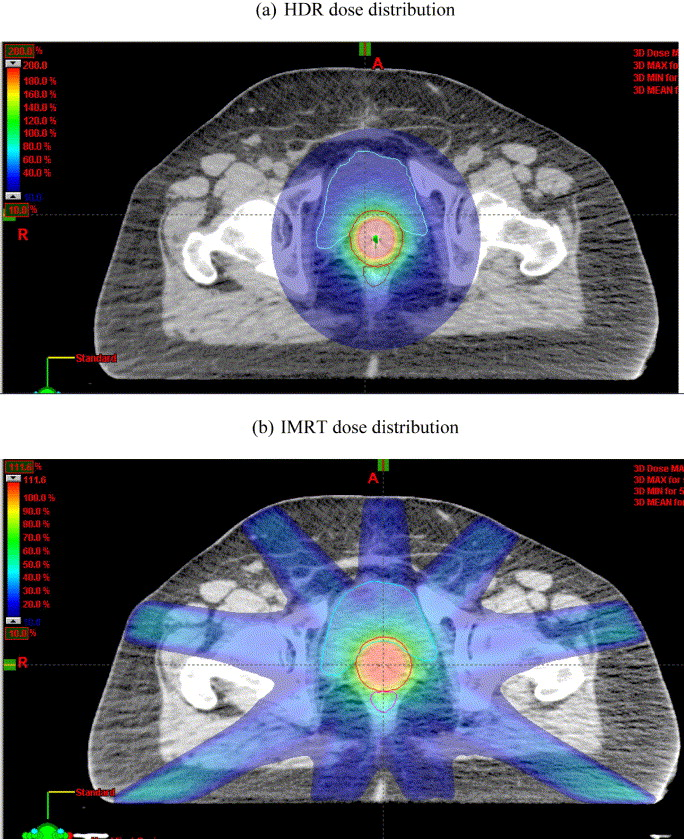
\includegraphics[width=8cm ]{images/imrt vs hdr.jpg}
    \caption{Image showing dose distribution targeting a tumour(red circle) using HDR(a) and IMRT(b)\cite{imrtVShdr}}
    \label{fig: imrtvshdr}
\end{figure}
\FloatBarrier 

\autoref{fig: imrtvshdr} shows the dose is spread throughout the body with \gls{imrt}, compared to \gls{hdr}, where the dose is centred near the tumour. The study concluded that \gls{imrt} provided a substantial decrease in dose delivered to the organs-at-risk near the tumour, compared to \gls{hdr}\cite{imrtVShdr}. \gls{imrt} is a viable treatment for treating tumours, but a large dose is still delivered to healthy tissue using this method. Furthermore, \gls{imrt} may not be a viable treatment option if the tumour is close to critical organs, such as the brain or heart.

\subsubsection{CT-scan}
\notinmain{kanskje nevn ein plass her om ka som er forventet av ein ideell proton terapi og korleis ein egentlig er i virkeligheten}
As mentioned before, \gls{ct}-scans are performed before \gls{rt}-treatment to calculate the body's radiodensity, which is the body's attenuation to radiation. These measurements are then used in dosage planning. It can also be used as a general imaging machine of a patient's insides, which can be used for diagnostics. A \gls{ct}-scan uses X-rays and computer technology to image a "slice" of the patient's body; many of these slice pictures are taken and put together to form a slice-by-slice model of the entire body of the patient.

A \gls{ct}-scan is normally realized with an X-ray tube that rotates around the patient that sends radiation through a slice of the patient. Sensors on the other side of the machine detect the photons as they leave the patient. \autoref{fig: ct_image} shows a typical setup when performing a \gls{ct}-scan.

 \begin{figure}[!htpb]
    \centering
    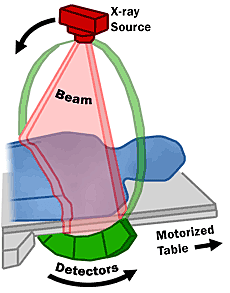
\includegraphics[width=8cm ]{images/CTXRAYScan.png}
    \caption{Image showing a typical setup for a CT-scanner\cite{CTimage}}
    \label{fig: ct_image}
\end{figure}
\FloatBarrier 

The photons from the X-rays lose their energy as they move through a medium, in this case, the patient. The energy loss from the photon is proportional to the density of the tissue. The detectors on the back of the patient measure the remaining energy of the photons exiting the patient and can, in turn, calculate the radiodensity of the path the photon travelled through the body.

Radiodensity measurements used in \gls{ct}-scans are measured in the Hounsfield-scale, which uses \gls{hu}. \gls{hu}, also called CT-unit, is a linear transformation of the absorption coefficient of the X-ray beam. 0 \gls{hu} is arbitrarily set to be the energy lost as the X-ray travels through water, and -1000 \gls{hu} is the energy lost when travelling through air. Using this unit, we measure the relative energy absorption of different tissues in body and use computer technology to reconstruct this information into a picture of the patient's insides. \autoref{fig: ct_lung_image} shows one slice from a \gls{ct}-scan performed on the patient's lungs.


 \begin{figure}[!htpb]
    \centering
    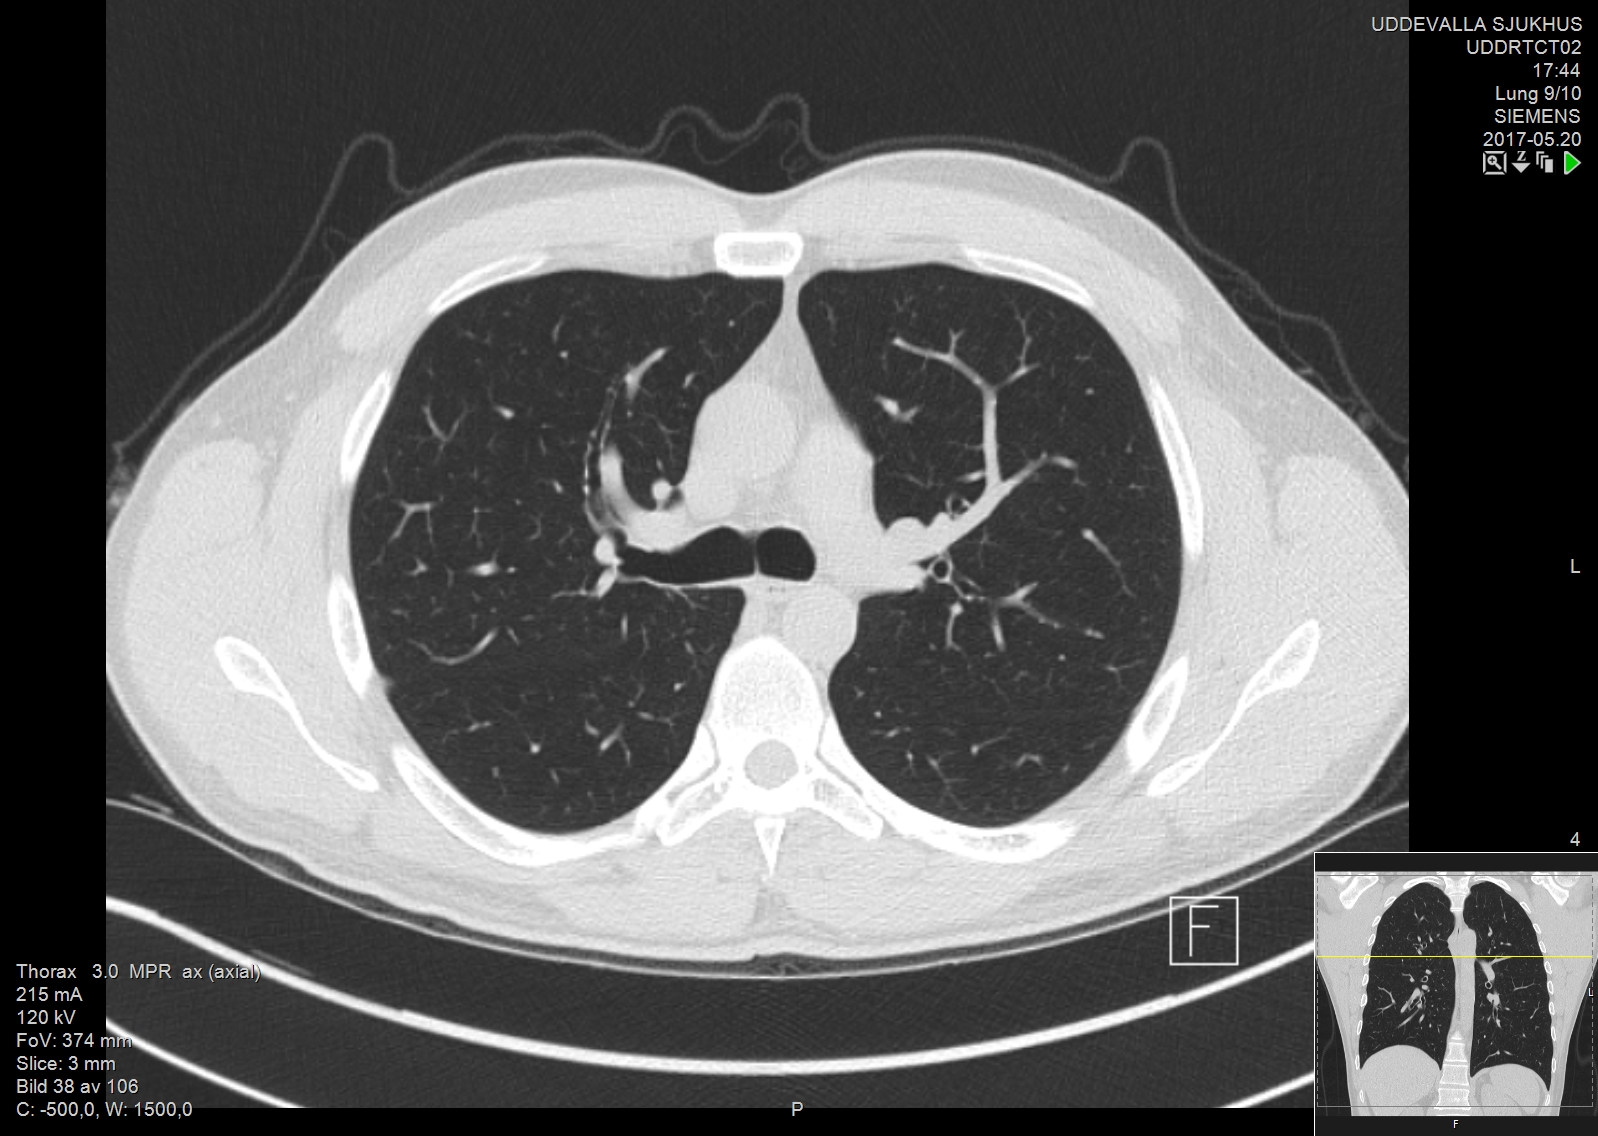
\includegraphics[width=12cm ]{images/High-resolution_computed_tomograph_of_a_normal_thorax,_axial_plane_(38).jpg}
    \caption{Image slice of a patient's lungs. Image down right of the image shows what slice of the lung is displayed. By Mikael Häggström, used with permission.}
    \label{fig: ct_lung_image}
\end{figure}
\FloatBarrier 


\subsection{Proton Therapy}

Particle therapy is a medical treatment similar to \gls{rt}, but instead of using X-rays to irradiate the body, high energy particles are used instead, the most common one today being protons. The idea for particle therapy came about in the mid 1900's, scientists discovered that, unlike photons, high energy particles do not deposit their energy gradually as it moved through a medium, rather it sharply deposited most of it one area. It was therefore theorized that proton therapy could be used as an alternative to \gls{rt}, to limit dose delivery to healthy tissue. 

\autoref{fig: bragg_peak} shows this sharp dose distribution of particles compared to the dose distribution of photons in tissue.

 \begin{figure}[!htpb]
    \centering
    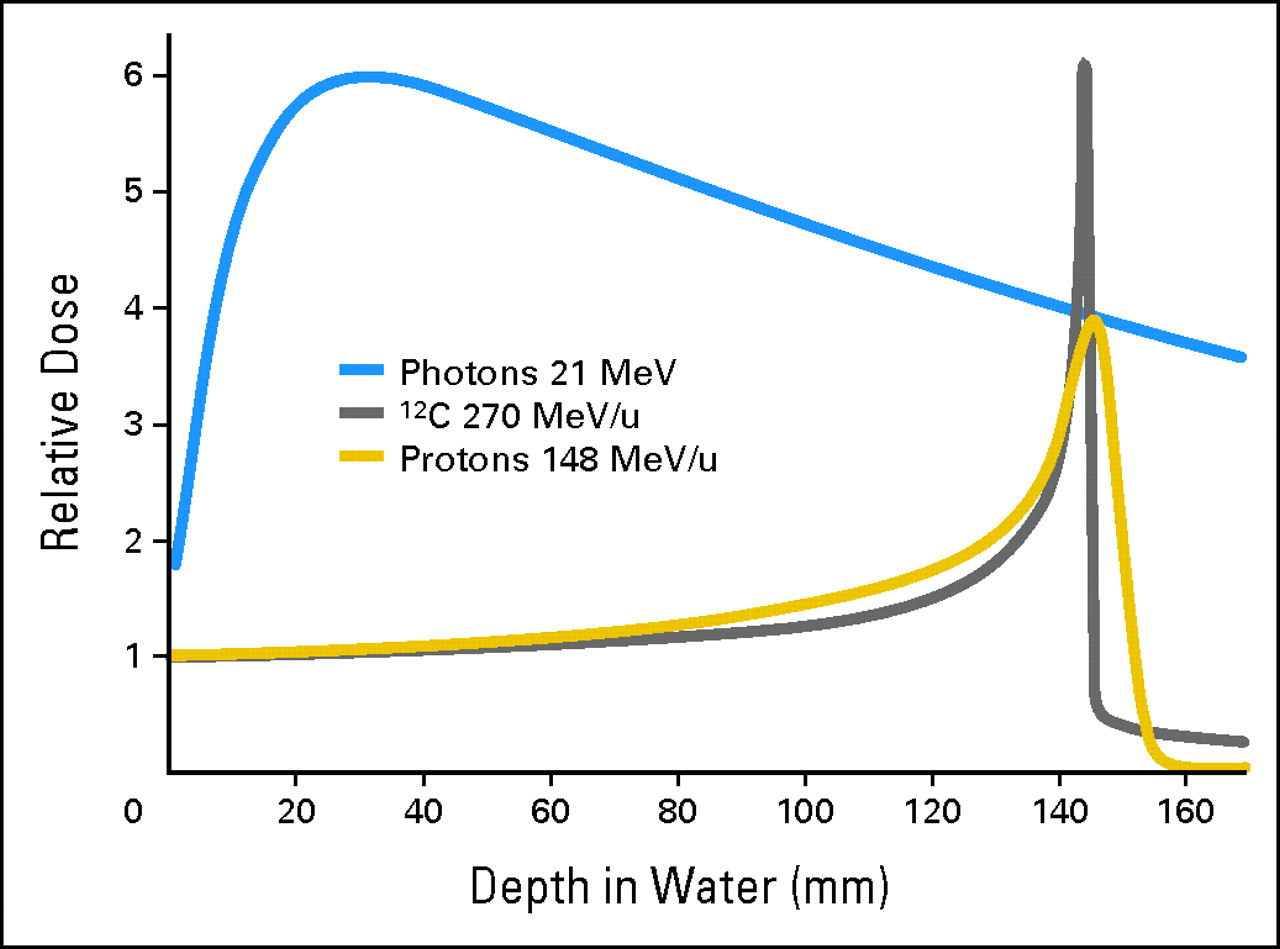
\includegraphics[width=10cm ]{images/bragg_peak.jpeg}
    \caption{Graph displaying the relative dose given in water by photons, protons and carbon-12 as function of distance. The bragg peak of proton and carbon-12 is shown to the right.\cite{bragg_peak_image}}
    \label{fig: bragg_peak}
\end{figure}
\FloatBarrier 

From the figure, photons reaches its max dose delivery early and slowly decreases as it is moving in the water. Protons have a relative low dose delivery until it reaches the bragg peak, where almost all energy is deposited. The reason protons deposit their energy is due to a phenomenon called "Bremsstrahlung", where the particle loses most of its energy as it is slowing down in the medium. To put in another way, the energy loss of a particle in a medium is inversely proportional to the velocity of the particle, leading to creating the bragg peak.

The effectiveness of proton therapy can be shown by comparing the dose delivered with conventional radiotherapy. \autoref{fig: imrt_vs_photon} compares the dose distribution of \gls{imrt} treatment and proton treatment of lung cancer in a patient.

\begin{figure}[!htpb]
    \centering
    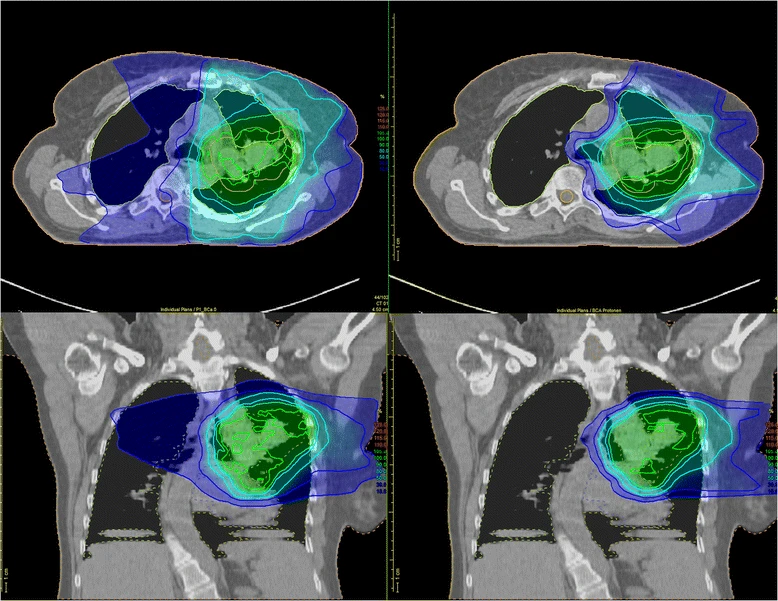
\includegraphics[width=12cm ]{images/proton_vs_imrt.png}
    \caption{Image showing the dose distribution of IMRT treatment(left) and proton therapy(right) of a a tumour in the lungs\cite{protonimage}}
    \label{fig: imrt_vs_photon}
\end{figure}
\FloatBarrier

One can clearly observe from the figure that \gls{imrt} irradiates a large part of tissue outside the tumour, as the entry and exit dose is high as predicted by \autoref{fig: bragg_peak}. In comparison, the proton treatment not only has a lower entry dose, but most of the radiation is limited to the area around the tumour. This allows us to irradiate the tumour with higher doses than what would be possible with photons, which gives us more effective treatments against cancers.

Proton therapy has potential as a treatment option, but it comes with its own challenges that must be tackled before beginning treatment. There are political and economical challenges with proton therapy,   . There is also the physics challenge; proton's nature as a particle means it behaves differently than photons. This means that dose and range calculations used for photons are insufficient for protons.\cite{proton_challenges}

Range uncertainties can have a major impact of proton therapy in comparison to \gls{rt}. \autoref{fig: proton_uncertainty} compares the dose distribution between radiation therapy and proton therapy, and how displays how range uncertainty can affect the distribution. The photons have a high entry dose and the dose delivered is reduced as photons travel deeper in the tissue. The proton dose is delivered by tuning the Bragg Peak of the beam to cover a small part of the tumour. After delivering a high dose, the beam is tuned again so the Bragg Peak covers another part of the tumour. This process is repeated until the entire tumour has been given a high dose. This creates a Spread Out Bragg Peak (SOBP) distribution, as shown in \autoref{fig: proton_uncertainty}.

\begin{figure}[!htpb]
    \centering
    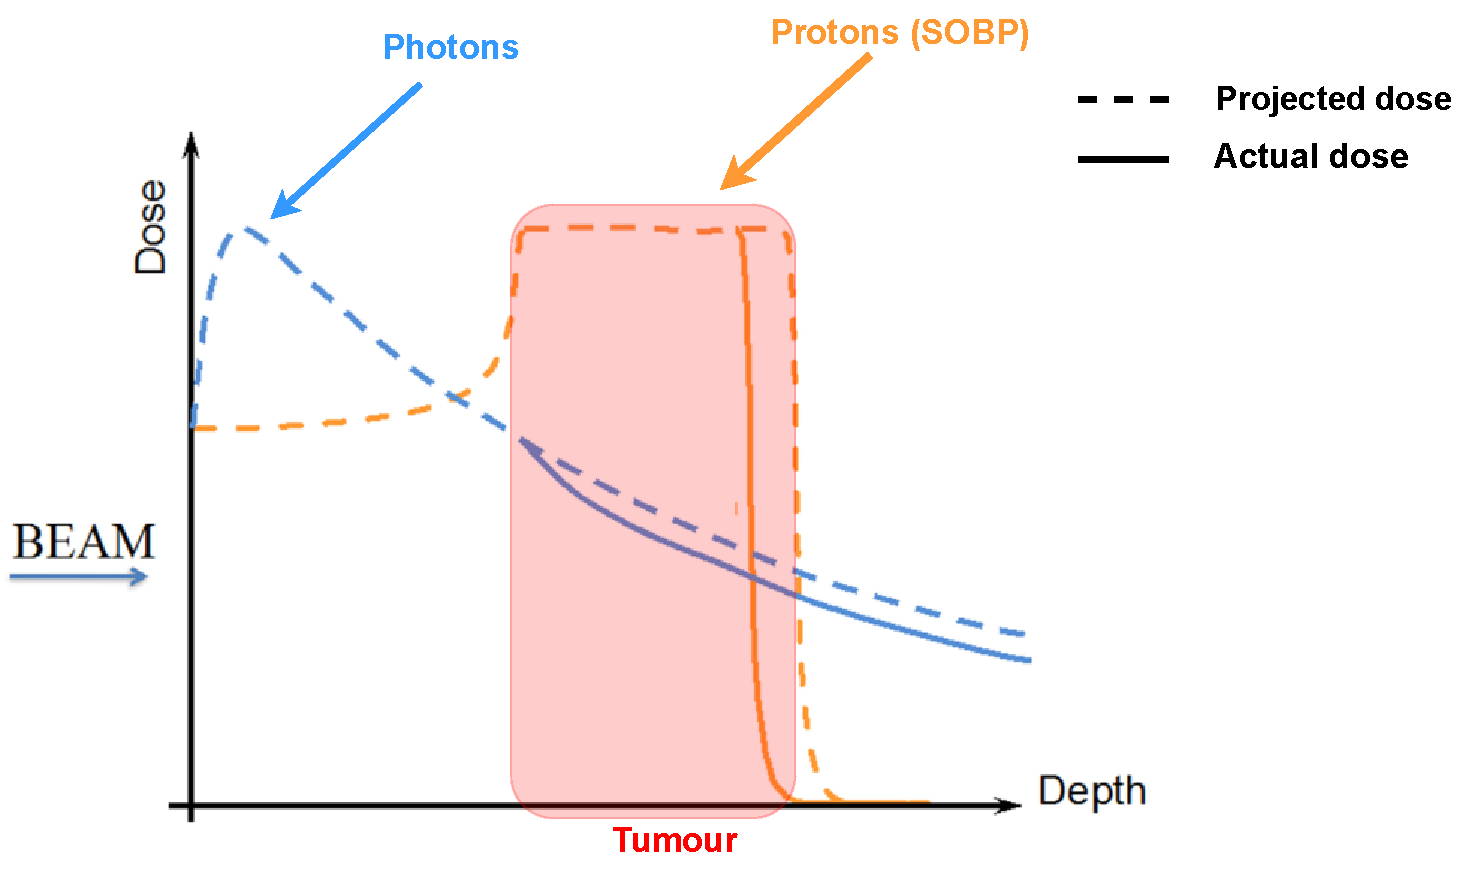
\includegraphics[width=12cm ]{images/projected_dose_graph.pdf}
    \caption{Image showing the effect of range uncertainties in photons(blue) and protons(orange)\cite{proton_challenges}}
    \label{fig: proton_uncertainty}
\end{figure}
\FloatBarrier


 The dotted lines is the projected dose to be delivered to the tumour and the full line is the actual dose delivered as a result of range uncertainties in the \gls{rsp} measurement. From the graph of the photons, we can see that, although there is a difference between the projected dose delivered and the actual dose, it does not impact the dose distribution in a significant way. The dose delivered to the tumour is approximately the same, regardless of the range uncertainties.
 
 For the protons, the deviation between the projected and actual dose is more severe. Because the dose delivery of the protons is much sharper, an undershoot in the dose delivery results in parts of the tumour not being covered by the Bragg Peak, and therefore almost no dose is delivered to it. Likewise, if there was an overshoot in the dose delivery, then healthy tissue could potentially enter the Bragg Peak, resulting in high irradiation of the tissue, which could cause harm to the patient. This illustrates that range uncertainty has a much bigger impact for proton therapy than in radiation therapy.

\notinmain{kanskje ha noken nummer på range uncertainty her}The range calculations for proton therapy is traditionally done by performing a \gls{ct}-scan of the patient and the \acrlong{hu}s from the scan is converted to \acrlong{rsp}. \gls{rsp} is a measurement of the stopping power of a particle moving through water, which can be used to estimate particle dose deliverance. The \gls{hu} measurement have an uncertainty to it, and although the uncertainty is not necessarily increased as one converts from \gls{hu} to \gls{rsp}, it will have a greater impact on particle therapy as opposed to \gls{rt}\cite{proton_challenges}.

A solution to avoid the uncertainty in the measurement is to measure the \gls{rsp} of the tissue directly, instead of converting it from \gls{hu}. This can be done by performing a \gls{ct}-scan with the same particle used for treatment, in this case a \acrfull{pct}-scan. \notinmain{fortsett med å snakke om gris-artikkelen og kanskje prøve å del opp meir av kapittelet i subsections/subsubsections}

By measuring \gls{rsp} directly with a \gls{pct}, it is expected to achieve a higher range precision than the conventional conversion method used with a normal ct-scan. A study was performed to test the accuracy of a \gls{pct}-scan versus a \gls{ct}-scan. A fresh post-mortem porcine structure was used to compare the \gls{rsp} measurement between a direct \gls{pct}-measurement, and the \gls{rsp} calculated from the \gls{ct}-scan.  \cite{porcine_2021}.

First, a measurement of the accuracy of the \gls{pct} was done by performing a \gls{pct}-scan of eight vials containing different tissue, shown in \autoref{fig: rsp_test}. The \gls{rsp} value of these different tissues was measured beforehand, with a multi-layered ionization chamber, and the \gls{rsp} values from that experiment is compared with the \gls{rsp} from the \gls{pct}-scan.

\begin{figure}[!htpb]
    \centering
    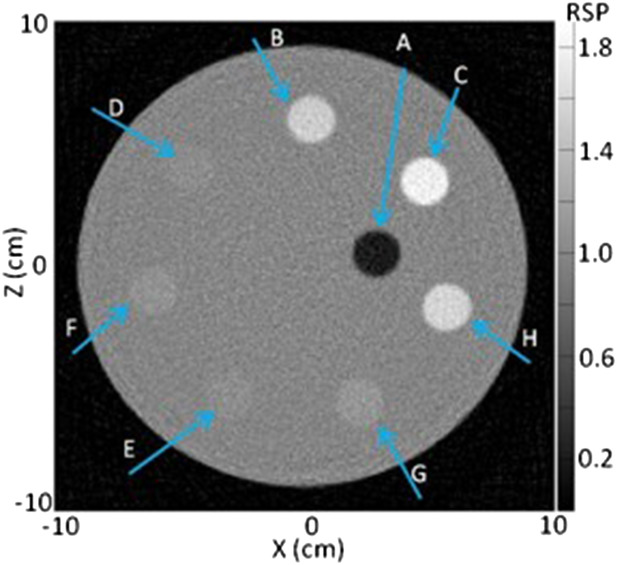
\includegraphics[width=8cm ]{images/porcine_phantom.jpg}
    \caption{Image of the RSP test done on several vials containing porcine tissue\cite{porcine_2021}}
    \label{fig: rsp_test}
\end{figure}
\FloatBarrier

The test revealed that there was up to 1\% difference between the \gls{rsp} measured with \gls{pct} and the results from the ionization chamber. There was an outlier of -4\% difference in the sinus tissue, but this can be caused by the low \gls{rsp} of the tissue along with the uncertainty of the \gls{pct} measurement. The range uncertainty from converting from \gls{hu} to \gls{rsp} has been shown to be at most 3.5\%\cite{Paganetti_2012}. This suggests that \gls{pct} yields higher accuracy measurements than a \gls{ct}-scan. 


Another test compared the calculated \gls{rsp} data from a \gls{ct}-scan, with the measured \gls{rsp} from a \gls{pct}-scan of the pig's head. The result is shown in \autoref{fig: porcine_pct_vs_ct}.

\begin{figure}[!ht]
    \centering
    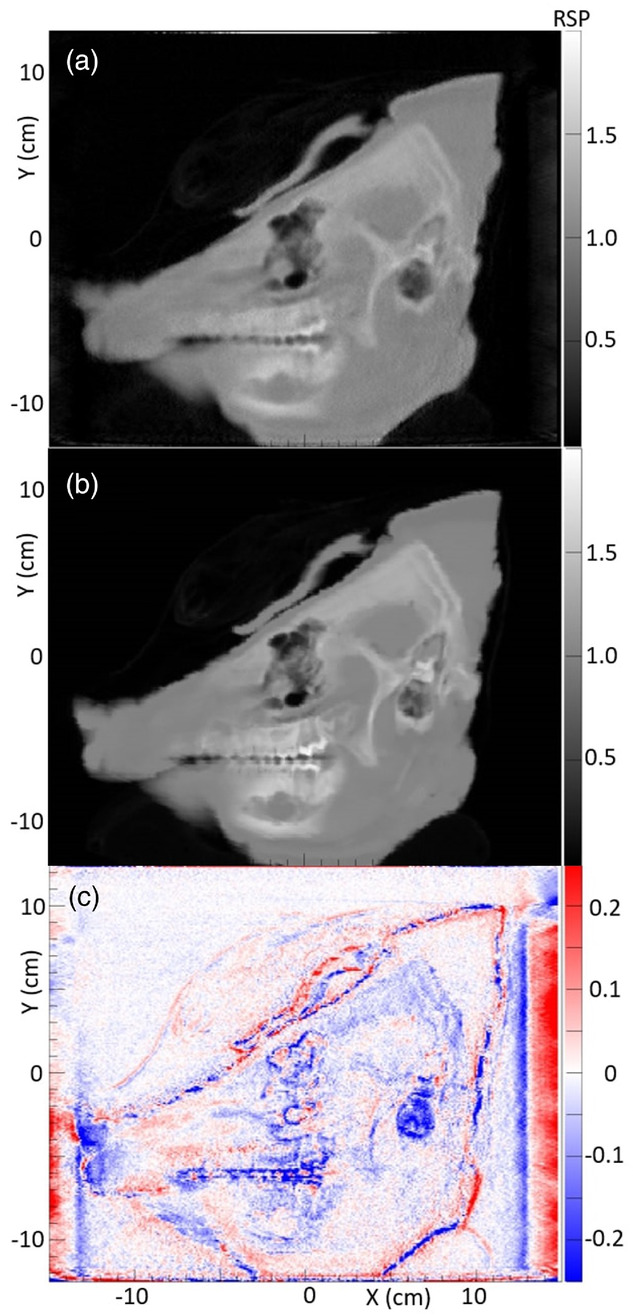
\includegraphics[scale=2.5]{images/porcine_comparison.jpg}
    \caption{Image showcasing difference between PCT and CT scan of the porcine head. (a) PCT. (b) CT. (c) difference between PCT and CT \cite{porcine_2021}}
    \label{fig: porcine_pct_vs_ct}
\end{figure}
\FloatBarrier

The data reveals that there is a relatively small difference between the calculated \gls{rsp} and the measured \gls{rsp} in soft tissue, with a difference at only 2\% between them. Structures such as teeth and bone shows larger discrepancies between them, up to a 30\% difference. The results from this test shows that there is a significant advantage to measure the \gls{rsp} value directly using \gls{pct} in comparison to calculating the \gls{rsp} values  it through converting Hounsfield-units This suggests scans of bone structures benefit more from using \gls{pct}. From this, we can conclude that \gls{pct} shows potential to outperform traditional \gls{ct} when measuring \gls{rsp} in a patient.

\end{document}